\documentclass{article}

\usepackage{ocencfd}
\usepackage{geometry}
\usepackage{graphicx}
\usepackage{float}
\usepackage{amsfonts}
\usepackage{mathrsfs}
\usepackage{mwe}
\usepackage{subfig}

\title{Introduction to Deep Learning\\Assignment 2} % Sets article title
\author{\textbf{Group 53}\\Chenyu Shi (s3500063); Shupei Li (s3430863); Shuang Fan (s3505847)} % Sets authors name
\documentID{Introduction to Deep Learning Assignment 2} %Should be alphanumeric identifier
\fileInclude{} %Names of file to attach
\date{\today} % Sets date for publication as date compiled
\graphicspath{{fig/}}
\geometry{a4paper, left=2cm, right=2cm, top=2cm, bottom=2cm}

% The preamble ends with the command \begin{document}
\begin{document} % All begin commands must be paired with an end command somewhere

\maketitle % creates title using information in preamble (title, author, date)

\section*{Task 1}

\section*{Task 2}
\setcounter{section}{2}
\subsection{Regression}
The regression model structure is shown in Figure \ref{fig:regression}. And its corresponding results are shown in Table \ref{tab:performance}. Because this is a regression task, we use MSE as loss function and Adam as optimizer. This model takes 2207593 trainable parameers, which is relatively high comparing to other models in task2. However, the final common sense loss is still a little bit high, which is 0.7053 hour(about 42.3 minutes). This is mainly caused by the problem of this kind of labels. Representing time in this way doesn't obey common sense. For example, 11:55 will be represented as 11.917 while 0:05 will be represented as 0.0833. Even though in common sense, the difference between 11:55 and 0:05 is only 10 minutes, their reformulated labels 11.917 and 0.0833 have a very high MSE. Therefore, this regression model has a limitted final performance.
\begin{figure}[!h]
	\centering
	\begin{minipage}[t]{0.3\textwidth}%并排放两张图片,每张占页面的0.5,下同。
		\centering
		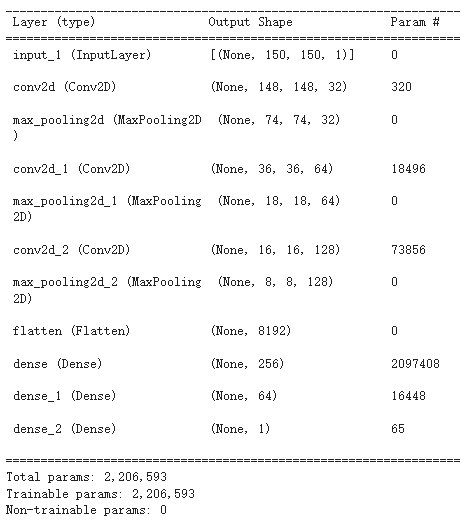
\includegraphics[width=\textwidth]{regression.png}
		\caption{Regression model}
		\label{fig:regression}
	\end{minipage}
	\begin{minipage}[t]{0.3\textwidth}%并排放两张图片,每张占页面的0.5,下同。
		\centering
		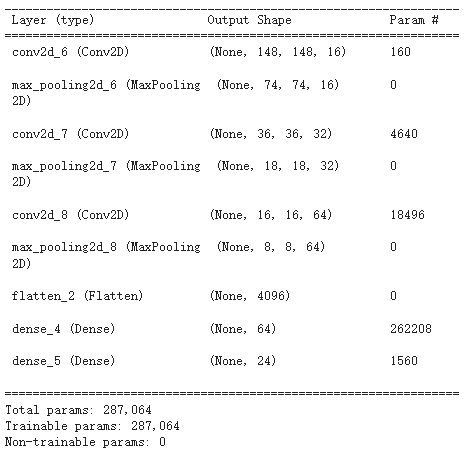
\includegraphics[width=\textwidth]{classification.png}
		\caption{Classification model}
		\label{fig:classification}
	\end{minipage}
	\begin{minipage}[t]{0.3\textwidth}%并排放两张图片,每张占页面的0.5,下同。
		\centering
		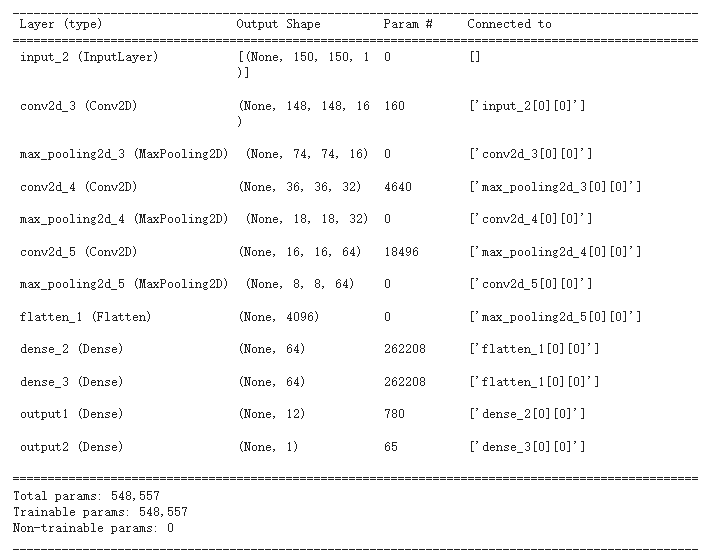
\includegraphics[width=\textwidth]{multi-head.png}
		\caption{Multi-head model}
		\label{fig:multi-head}
	\end{minipage}
\end{figure}
    \begin{table}[!ht]
	\caption{Results and Algorithm Comparison}
	\label{tab:performance}
	\centering
	\begin{tabular}{cc}
		\toprule
		\textbf{Model} & \textbf{Common Sense Loss(hours)} \\
		\midrule
		Regression & 0.7053 \\
		Classification(24 classes) & 0.6206 \\
		Classification(72 classes) & 0.9517 \\
		Classification(720 classes) & 3.0309 \\
		Multi-head & 0.6161 \\
		Label transformation & 0.3447 \\
		Label transformation(fine-tuned) & 0.1921 \\
		\bottomrule
	\end{tabular}
\end{table}
\subsection{Classification}
The regression model structure is shown in Figure \ref{fig:classification}. And its corresponding results are shown in Table \ref{tab:performance}. Thereinto, model structures of 24 classes, 72 classes and 720 classes are only different in last output layers. Because this is a multi-class classification task, we use cross entropy as loss function and Adam as optimizer. And we can see, although classification model uses much fewer trainable parameters(for 24 classes, 287064 trainable parameters), the final result for 24 classes is better than regression model with a performance of 0.6206 hours(about 37.2 minutes). However, when we increase the number of categories, the performance of model become poorer. And the model of 720 classes even didn't coverge and has a very high common sense loss. That's because this kind of label representation also has its problems. The first problem is that this label representation cannot measure "how much difference two categories have". For example, in 24 classes model, 0:01 and 0:31 are in different categories, and 0:01 and 6:00 are also in different categories. Although the common sense loss between 0:01 and 6:00 are much larger than that between 0:01 and 0:31, the cross entropy loss function in classfication task will give them same loss values. The second big problem is that it's hard for us to balance  sampling interval and samples number. If we have large sampling interval along with a large samples number, the model can get well trained because there are sufficient training data in each class, but the common sense loss within each class becomes rather high. For example, in 24 classes model, 0:01 and 0:29 will be classified into same class even they are almost half an hour apart. On the contrary, if we have small sampling interval along with a small samples number, the common sense loss within each class becomes rather small, but the model itself cannot be well trained due to lack of training data for each class. For example, in 720 classes model, each class will only have 25 pictures for training, validation and test set. That's not a sufficient number for training CNN in a regular way.

\subsection{Multi-head}
The regression model structure is shown in Figure \ref{fig:multi-head}. And its corresponding results are shown in Table \ref{tab:performance}. We use two heads output, one for predicting hours and another for predicting minutes, and we consider these two heads output as multiclass classification task and regression task respecitively. For classification task of predicting hours, we consider 12 hours as 12 different categories and use cross entropy as loss function. For regression task of predciting minutes, we use MSE as loss function. And this model uses 548,557 tranable parameters and finnaly obtains common sense loss of 0.6161 hours(about 37.0 minutes), which is the best performance up to know comparing to regression and classification models. The performance improvement is due to that using multi-head model can take adavantage of different features of the target labels. For example, for target of predicting hours, it's a good way to consider it as a classification task because there are only 12 classes and each class can have adequate training samples. On the contrary, for target of predicting minutes target, it's a good way to consider it as a regression task because the target values are in a rather large interval(0-59). It's flexible to use multi-head model to combine these features using different losses and targets, so the final performance can be improved. Besides, there's an important thing needed to pay attention to. That is for regression task, we should scale and normalize predicting target from interval (0-59). For example, divide 60 for each minute target. Otherwise, the cross entropy loss for hours and the MSE loss for minutes will have great difference in quantity, which has negative impact on training neural networks. Howerver, although multi-head has gained performance improvement, the problems of labels of classification and regression tasks are still there. Therefore, in the next subsection, we will use Label transformation to improve model and get much better results.


\subsection{Label transformation}
According to the performance of previous model, we can know that directly using hours and minutes as target cannot capture common sense loss, which has negative influence on the model performance. Therefore, we use sine and cosine functions to represent the angles on the unit circle to improve the model performance.

It's easy to think that the angle of hour hand $\theta$ contains entire information about the clock. Then we apply sin function on that angle $\theta$. Now let's see the difference of previous example, 0:05 and 11:55. It's simple to compute the corresponding angles of 0:05 and 11:55, which are 0.0436 rads and 6.240 rads. And we could see, sin(0.0436) and cos(6.240) equals to 0.0436 and -0.0436 respectively, which are very close to each other due to the property of periodic function. It's exactly what we want for our labels.

But there is another problem. For sin function, there are many angles, or clock time, are projected to a smae value. For example, 1:00($\frac{\pi}{6}$) and 5:00($\frac{5\pi}{6}$) are both projected to 0.5. Luckily, we could apply cos function at the same time to distinguish these angles. Therefore, we should transform the original label [hour,minute] to [sin($\theta$),cos($\theta$)]. So the output nodes should be 2, one for sin, and another for cos. We know sin and cos function both have a range of [-1,1]. And we know tanh activation function has the same range. Therefore, applying a tanh activation function in the output layer would be perfect. And we consider it as a regression problem as well.
\begin{figure}[!h]
	\centering
	\begin{minipage}[t]{0.3\textwidth}%并排放两张图片,每张占页面的0.5,下同。
		\centering
		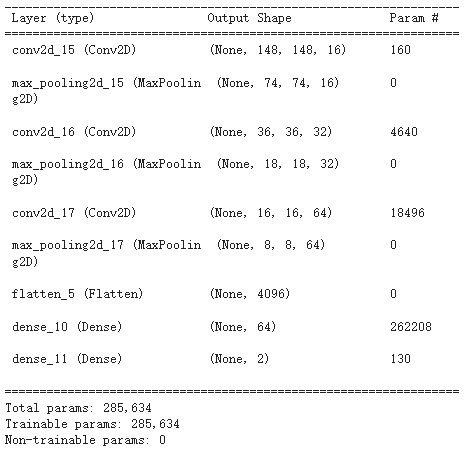
\includegraphics[width=\textwidth]{label_trans.png}
		\caption{Label transformation model}
		\label{fig:labeltrans}
	\end{minipage}
	\begin{minipage}[t]{0.3\textwidth}%并排放两张图片,每张占页面的0.5,下同。
		\centering
		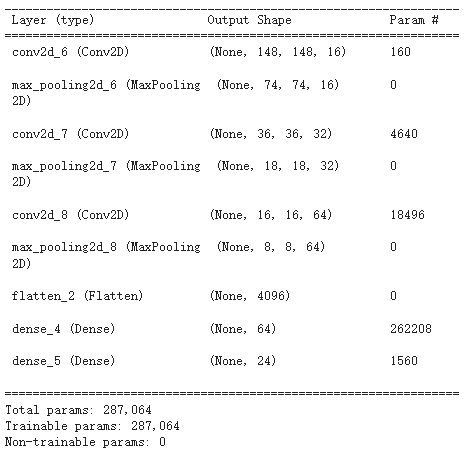
\includegraphics[width=\textwidth]{classification.png}
		\caption{Final model}
		\label{fig:final}
	\end{minipage}
\end{figure}

This label transformation regression model works well. The specific model structure and model performance are shown in figure \ref{fig:labeltrans} and table \ref{tab:performance} respectively. It only takes 285634 trainalbe parameters and obtain common sense loss of 0.3447 hours(about 20.7 minutes), which is the best up to now. In the next section, we will fine tune this model using the knowledge gained by previous part and improve its performance as the final model.

\subsection{Final model}

The final model structure and its performance are shown in figure \ref{fig:final} and \ref{tab:performance} respectively. Comparing to the model in section 2.4, we made several adjustments. Firstly, we use leakyrelu instead of relu as activation function in all hidden layers to avoid vanishing gradient problem. In addition, we apply L2 regularization for each layer that contains trainable parameters to avoid overfitting. Besides, a dropout layer is applied after flatten and a normalization layer is applied after the first dense layer. Finally, we set checkpoints to store the model with best performance on validation set, and use a smaller learning rate and large total epochs.

The final performance obtained by this model is common sense loss of 0.1921 hours(about 11.5 minutes), which is the best one among all, especially comparing to the first three models. That's mainly because periodic functions sin and cos can exactly capture the common sense loss of clock time. To conclude, from this experiments we can see, it's of much importance to design a good target label for neural networks to train and obtain a rather good final performance.
Also, we could see a fine-tune can improve model's performance as well.
\section*{Task 3}
\setcounter{section}{3}
\subsection{Datasets}
We use two datasets in Task 3. Firstly, we explore the performance of different model architectures and the effects of different parameters with MNIST data. After that, we leverage the power of generative models on Butterfly \& Moth data. \par
We directly call Tensorflow API to download the MNIST dataset. However, the original dataset is also available on \url{https://deepai.org/dataset/mnist}. MNIST dataset contains 70,000 grayscale images (28 $\times$ 28 $\times$ 1), whose content is handwritten numbers. \par
Butterfly \& Moth is an open source dataset on Kaggle. There are 13,639 RGB images (224 $\times$ 224 $\times$ 3) composed of 100 butterfly or moth species. Link of the dataset is \url{https://www.kaggle.com/datasets/gpiosenka/butterfly-images40-species?resource=download}.

\subsection{Experimental Set-up}
All experiments are deployed on two servers. Server 1 has an Intel(R) Xeon(R) Platinum 8358P CPU and a RTX A5000 GPU, while server 2 has an Intel(R) Xeon(R) E5-2680 v4 CPU and a TITAN Xp GPU. Table \ref{tab:3-hyper} summarizes the hyperparameter values in the experiments. The following describes the process of our experiments.
\begin{table}[!ht]
    \centering
    \caption{Hyperparameter Settings}
    \label{tab:3-hyper}
    \begin{tabular}{lll}
        \toprule
        \textbf{Parameter} & \textbf{Value} & \textbf{Meaning}\\
        \midrule
        cae\_latent\_dim & 32 & Dimensions of the latent space in CAEs.\\
        cae\_epoch & 10 & The number of training epochs in CAEs.\\
        vae\_latent\_dim & 32 & Dimensions of the latent space in VAEs.\\
        vae\_epoch & 20 (MNIST) / 100 (Butterfly \& Moth) & The number of training epochs in VAEs.\\
        gan\_latent\_dim & 256 & Dimensions of the latent space in GANs.\\
        gan\_epoch & 20 (MNIST) / 250 (Butterfly \& Moth) & The number of training epochs in GANs.\\
        \bottomrule
    \end{tabular}
\end{table}

\subsubsection{MNIST}
We modify the model architecture to decrease the model complexity and match the data better. Specially, we build the basic convolutional network with four Conv2D layers and construct the basic deconvolutional network with one Conv2DTranspose layer. Figure \ref{fig:3-model} illustrates our model settings. There is no need to resize the images due to the modification of the model.
\begin{figure}[!ht]
    \centering
    \subfloat[Convolutional network]{%
        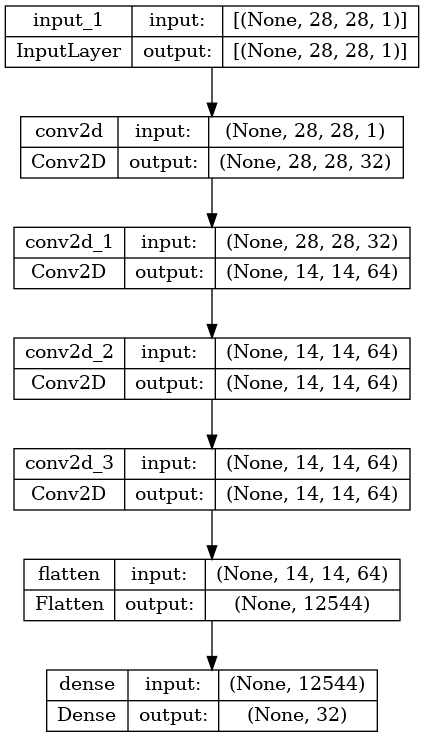
\includegraphics[height=6cm, width=6cm]{./fig/conv.png}%
        \label{fig:conv}%
        }%
        \hspace{0.8cm}
    \subfloat[Deconvolutional network]{%
        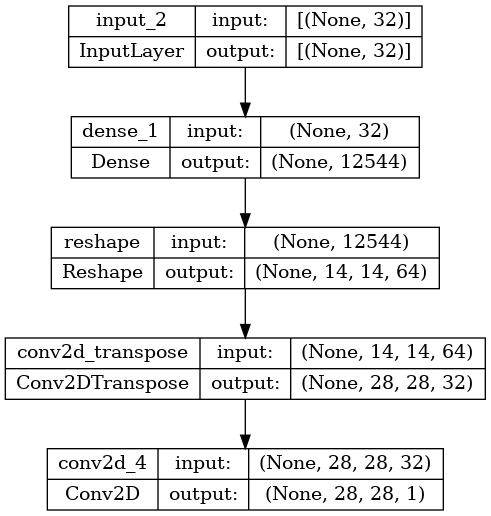
\includegraphics[height=6cm, width=7cm]{./fig/deconv.png}%
        \label{fig:deconv}%
        }%
    \caption{Model Structure}
    \label{fig:3-model}
\end{figure}

\subsubsection{Butterfly \& Moth}
We rescale the images to 64 $\times$ 64 $\times$ 3 and directly apply the model architecture provided in the notebook when working with Butterfly \& Moth data.

\subsection{Results}
\textbf{CAEs}. Figure \ref{fig:3-cae} shows the reconstructed images from CAEs. It is easy to see that CAEs have captured the main features in the original images.
\begin{figure}[!ht]
    \centering
    \subfloat[MNIST: Original Images]{
        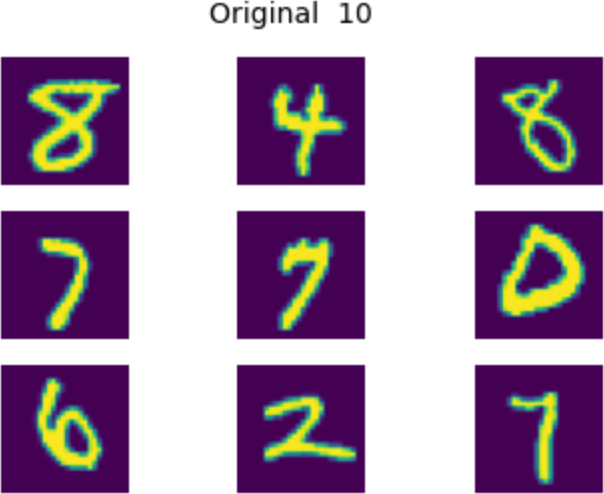
\includegraphics[width=5.6cm]{./fig/mnist-cae-ori.png}
    }
    \hspace{1cm}
    \subfloat[MNIST: Reconstructed Images]{
        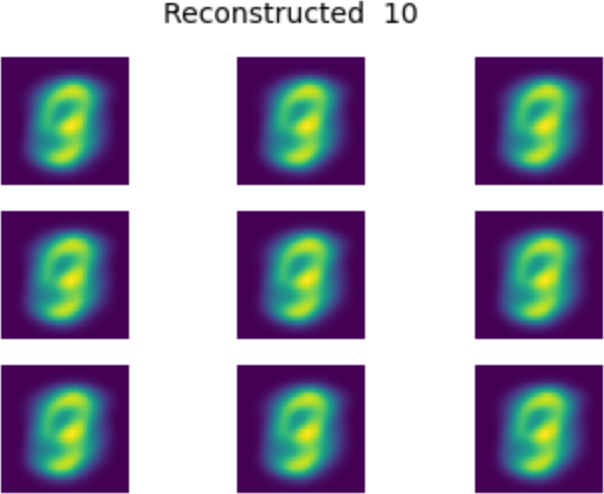
\includegraphics[width=5.6cm]{./fig/mnist-cae-re.png}
    }
    \\
    \subfloat[Butterfly \& Moth: Original Images]{
        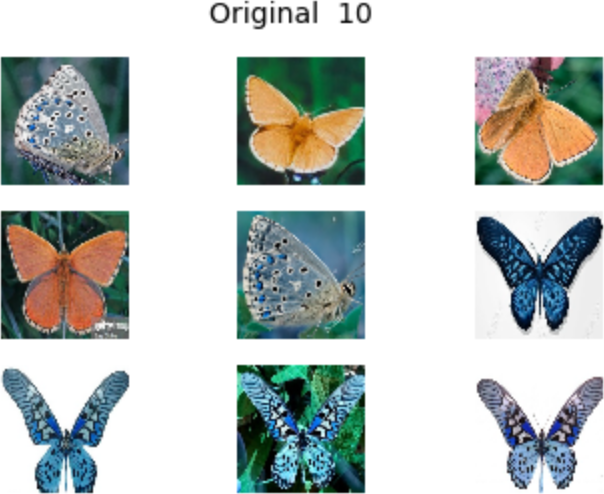
\includegraphics[width=5.6cm]{./fig/bm-cae-ori.png}
    }
    \hspace{1cm}
    \subfloat[Butterfly \& Moth: Reconstructed Images]{
        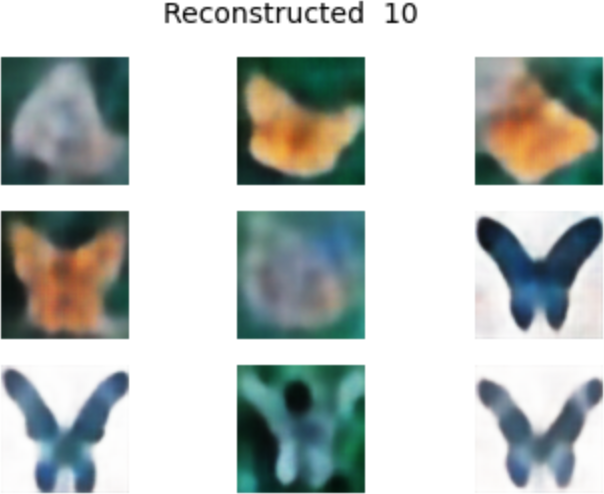
\includegraphics[width=5.6cm]{./fig/bm-cae-re.png}
    }
    \caption{Results of CAEs}
    \label{fig:3-cae}
\end{figure}
\par~\\
\textbf{VAEs}. We explore the learned latent space with linear interpolation technique. Firstly, we sample a point from the latenty space by generating its coordinates from a standard normal distribution. Then, we change one or two coordinates along the straight line in the latent space, while keep other coordinates unchanged. For MNIST dataset, we apply linear interpolation on the 10th and 27th coordinates simultaneously, which are related to the shape of the number. Figure \ref{fig:vae-mnist} shows the visualization results.
\begin{figure}[!ht]
    \centering
    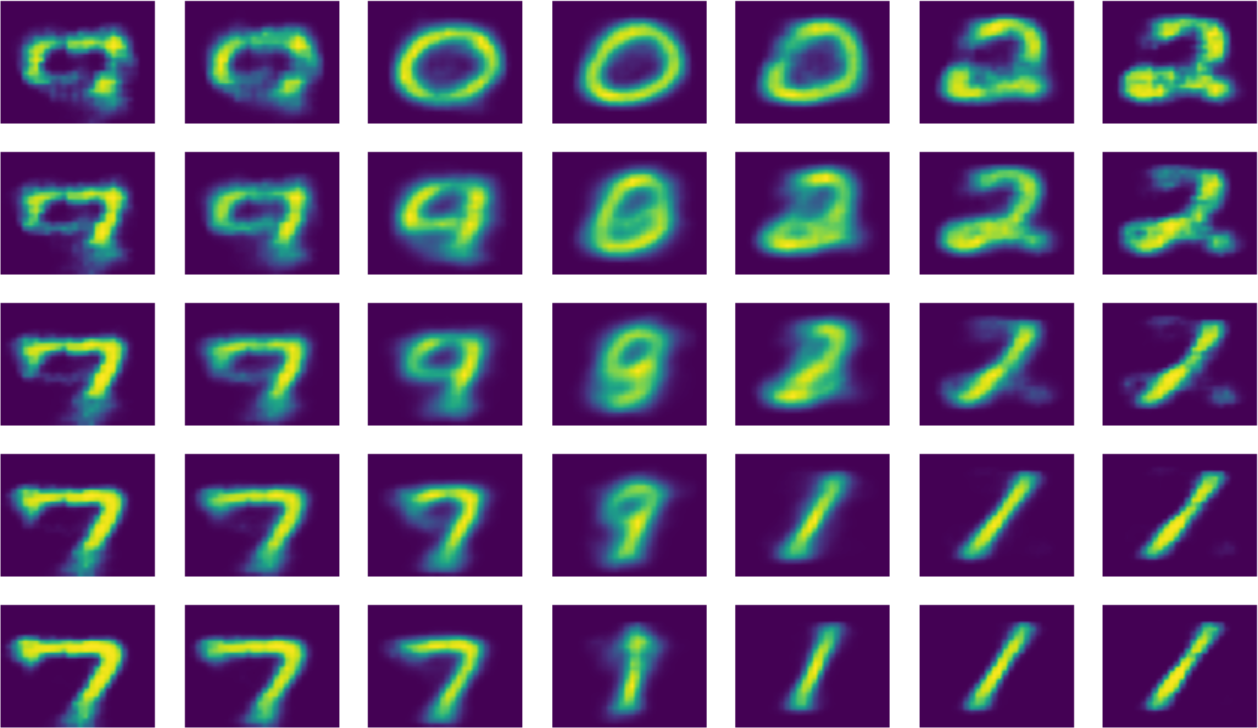
\includegraphics[width=10cm, height=5cm]{./fig/mnist-vae.png}
    \caption{VAEs: MNIST Data}
    \label{fig:vae-mnist}
\end{figure}
As for Butterfly \& Moth data, we linearly interpolate the 6th and 29th coordinates, whose outputs are presented in Figure \ref{fig:vae-bm}. According to Figure \ref{fig:vae-bm}, the 6th coordinate is related to the color of wings, while the 29th coordinate is concerned with the width of wings.
\begin{figure}[!ht]
    \centering
    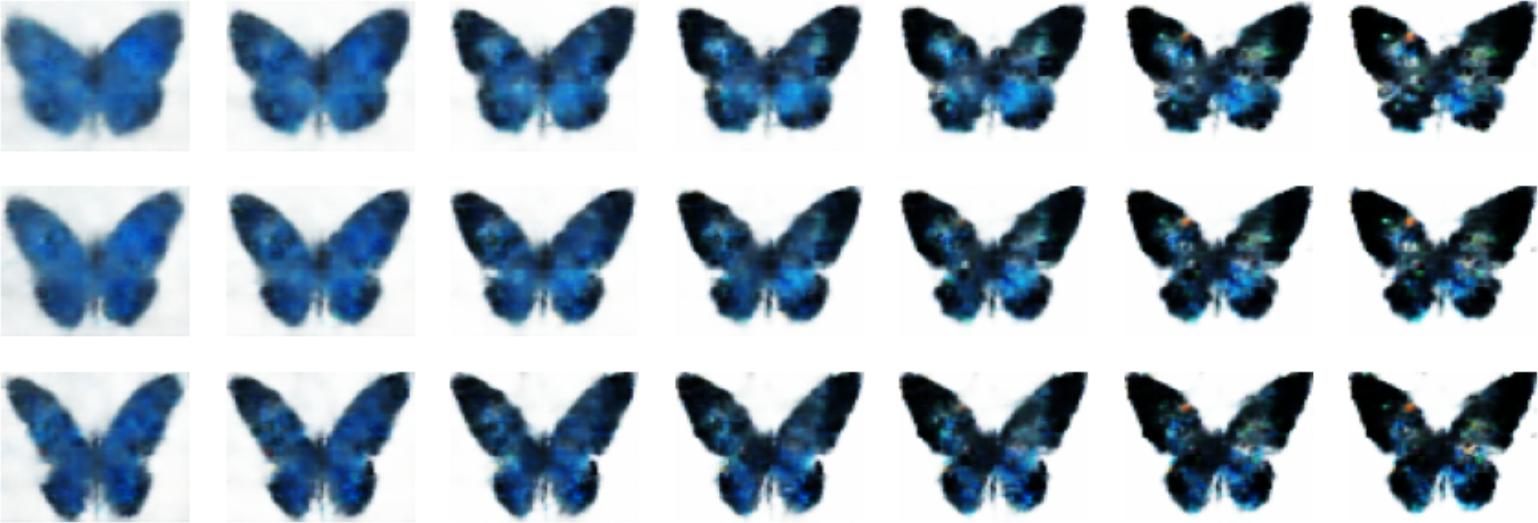
\includegraphics[width=10cm, height=4cm]{./fig/bm-vae.png}
    \caption{VAEs: Butterfly \& Moth Data}
    \label{fig:vae-bm}
\end{figure}
\par~\\
\textbf{GANs}. We visualize the outputs of linear interpolation in the same way as VAEs. We change the 1st, 120th, and 126th coordinates for MNIST data to obtain different numbers. Figure \ref{fig:gan-mnist} shows the generated images. For Butterfly \& Moth data, we change the 40th coordinate, which is related to the color and the posture of the butterfly. Figure \ref{fig:gan-bm} shows the generated butterfly.
\begin{figure}[!ht]
    \centering
    
\includegraphics[width=10cm, height=1cm]{./fig/gan-1.png}
    
\includegraphics[width=10cm, height=1cm]{./fig/gan-2.png}
    
\includegraphics[width=10cm, height=1cm]{./fig/gan-3.png}
    \caption{GANs: MNIST Data}
    \label{fig:gan-mnist}
\end{figure}
\begin{figure}[!ht]
    \centering
    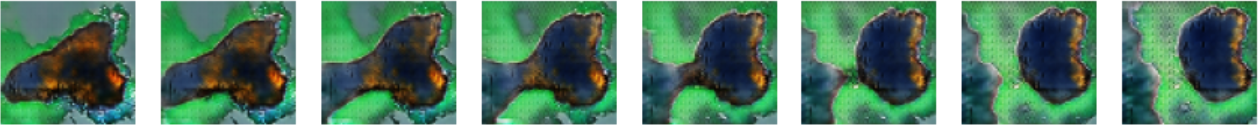
\includegraphics[width=10cm, height=1cm]{./fig/gan-bm.png}
    \caption{GANs: Butterfly \& Moth Data}
    \label{fig:gan-bm}
\end{figure}

\subsection{Discussion: Model Comparison}
CAEs are autoencoders that apply the CNN architecture to compress the input images into a lower dimensional latent space and reconstruct the images from the learned latent space. Using an encoder/decoder structure enables CAEs to capture as much information about data as possible, even without labels. However, CAEs are deterministic. That means there is a one-to-one relationship between the input and output in CAEs. Therefore, CAEs can't generate new samples. Based on the architecture of the traditional autoencoder, VAEs introduce randomness into the model by assuming a prior distribution of latent space and infering the posterior distribution during the training process. In most cases, we choose the standard Gaussian distribution as prior distribution, which helps the latent space to be complete and continuous. The probabilistic nature allows VAEs to generate new images from random noise.\par
GANs are designed for generating new samples. Instead of inferring the distribution of latent space, GANs sample from random noise and learn a transformation to imitate the real distribution of data. Gans improve the quality of imitations by training a discriminator to distinguish between generated samples and real samples.\par
In summary, VAEs sample from a prior distribution and infer the real distribution of latent space, while GANs sample from random noise and learn the data transformation by encouraging the competition between generator and discriminator.

\section*{Contributions}
\begin{tabular}{ll}
    \textbf{Name} & \textbf{Contribution}\\
    Chenyu Shi & Task 1 code, Task 2 code, Task 2 report.\\
    Shupei Li & Task 3 code, Task 3 report, Task2 code.\\
    Shuang Fan & \\
\end{tabular}
\end{document}
